\documentclass[conference]{IEEEtran}



\ifCLASSINFOpdf
\else
\fi



\usepackage{url}
\usepackage{graphicx}
\usepackage{float}
\usepackage{hyperref}
\usepackage[table]{xcolor}
\hyphenation{op-tical net-works semi-conduc-tor}


\begin{document}

\title{Prediction of Accurate Occupancy in an office 
room using Supervised Machine Learning 
Techniques}


% author names and affiliations
% use a multiple column layout for up to three different
% affiliations
\author{\IEEEauthorblockN{Mina Moghaddam}
\IEEEauthorblockA{Engineering Faculty\\ Department of Computer Engineering\\
			Middle East Technical University\\
			Ankara, Turkey\\
			Email: Mina.moghaddam90@gmail.com\\
			Student Number: 2343341}
\and
\IEEEauthorblockN{Tahsincan K{\"o}se}
\IEEEauthorblockA{Engineering Faculty\\ Department of Computer Engineering\\
			Middle East Technical University\\
			Ankara, Turkey\\
			Email: tahsincan.kose@ceng.metu.edu.tr\\
			Student Number: 2188423}
\and
\IEEEauthorblockN{M. Rasit Ozdemir\\  Engineering Faculty}
\IEEEauthorblockA{Department of Computer Engineering\\
            Middle East Technical University\\
            Ankara, Turkey\\
            Email: e1942606@ceng.metu.edu.tr\\}
\and
\IEEEauthorblockN{\ \ \ \ \ \ \ \ \ }
\IEEEauthorblockA{\ \ \ \ \ \ \ \ \ }
\and
\centering
\IEEEauthorblockN{Zakiah Utami}
\IEEEauthorblockA{Engineering Faculty\\ Department of Computer Engineering\\
			Middle East Technical University\\
			Ankara, Turkey\\
			Email: utami.zakiah@metu.edu.tr\\
			Student Number: 2102663}
}




% make the title area
\maketitle

% As a general rule, do not put math, special symbols or citations
% in the abstract
\begin{abstract}
The abstract goes here.
\end{abstract}



\section{Introduction}
In this era, occupation in human spaces impress different aspects of a building like light, temperature, humidity and so on. In order to meet this needs heating, cooling and ventilation are required. These accounts for 35\% energy usage in the United States. Currently, most modern
buildings still condition rooms assuming maximum occupancy rather than actual usage.It is of little debate in today’s world that modeling occupant behavior and its information is of great importance. It is quite expected to notice significant energy savings that can be achieved by the accurate prediction of occupancy in buildings. In this developed society, commercial office buildings require large amount of area and energy to create comfortable zone for their occupants. In detail lighting, heating, ventilation and
air-conditioning systems (L-HVAC) consume the most energy,
together accounting for about 70\% of the overall energy consumed in
a typical office building\cite{OccMeasure}. With this in mind, the office buildings are useful targets of modeling occupant behavior to manage its potential of energy sources accurately in order to increase energy savings. In a recent study it is illustrated that accurate occupation prediction in buildings has been estimated 15 to 25\% energy savings \cite{ReductoHVAC}. In another simulation-based study\cite{SensorOcc}, the potential energy savings is suggested as approximately 30\%.\\

Current status of industrial energy consumption possess an important risk to society and environment in terms of sufficiency of resources. Although various governments around the globe have set quantified targets that anticipate 20\%\cite{TargetCons} energy usage reduction in overall, the total industrial consumption still follows an ascending trend. Also, commercial office buildings comprise the majority of in floor areas in most of the developed countries hence consume remarkable amount of energy in the logistics of building services. Having all these considered, the problem regards to the necessity of effective energy usage. Meanwhile, this implies the minimization of resource dissipation in such enormous in-floor areas. In fact, this is just a single part of the whole problem. Thinking on a global scope brings one to the problem of world's inability to restore its natural resources fully anymore. Failing to capture this problem would result in higher energy wastage which becomes more and more profoundly threatening for the entire world. For that reason, resolving this sub-problem effectively would inspire all other sectors, thus affects the whole problem in long term.

\section{Method}
The project's aim is to predict occupation in an office room during different hours based on the data from light, temperature, humidity and CO2 by using Machine Learning approach. There were used three datasets for training and testing, that two testing datasets for open and close door in the office \cite{Candanedo}.


The original article in which the dataset was gathered and analyzed used a variety of statistical approaches on the data. The authors of the original article have named 4 of the methods in which they have better results: Random Forest (RF), Linear Discriminatory Analysis (LDA), Classification and Regression Trees (CART), and Gradient Boost Machines (GBM), but they have tried other methods such as Artificial Neural Networks (ANN) and Support Vector Machines (SVM) \cite{Erickson}. Our aim is to take ANN, SVM or a combinatory approach of both methods. Additionally, we assume that augmenting the data with expert knowledge extracted from the already existing dataset can have a boosting effect on performance of our method.

The datasets consist of labeled training and test data (for supervised learning) with 7 attributes such as Time (Date time: year-month-day hour: minute: second), Temperature (Celsius), Relative Humidity (\%), Light (Lux), CO2 (ppm), Humidity Ratio (Derived quantity from temperature and relative humidity, in kg water-vapor/kg-air) and Occupancy (0 or 1, 0 for not occupied, 1 for occupied status). Training data consists of 8143 entities. Test data is divided into two portions, one is data gathered while the door was close, with 2665 rows of data, and the other one is data gathered while the door was open, with 9752 rows of data \cite{Ryu}.

We have used the already existing information to augment the data with 9 new attributes. These 9 new attributes are: Differences of CO2 level in 1 minute interval, Differences of CO2 level in 3 minutes interval, Differences of CO2 level in 5 minute interval, Differences of Humidity level in 1 minute interval, Differences of Humidity level in 3 minute interval, Differences of Humidity level in 5 minute interval, Differences of Light level in 1 minute interval, Differences of Light level in 3 minute interval, and Differences of Light level in 5 minute interval.

This approach is to globalize the model. The previous study \cite{Pedersen} have used absolute values which can be attributed to a certain location or time. By training a model using only the difference we are assuming the model will become more invariant to time and location.


\section{Evaluation}
Before anything, it is highly beneficial to make descriptive analysis on the data rather than throwing it into models. For this purpose, visualizing data is a good first practice. Recalling that the dataset is processed, it now constitutes of 9 attributes which require a hyperplane representation. In order to have a decent visualization, reducing the parameter space to 2 and 3 most important ones (only for visualization) using \textit{Feature Selection}\cite{Guyon} is a common method. However, feature selection might not provide a clear separation between the distinct classes. Such a separation heavily depends on the complexity of data. \textit{\textbf{sklearn}} library is used throughout the model setups in the course of feature manipulation tasks in which all these are readily implemented to facilitate one-line usages. For instance, \textbf{K} best features in terms of \textit{\textbf{chi square}}\cite{Fahim} independence (relatedness) score metrics are extracted through utilization of aforementioned library. All in all, best features are plotted in a scattered manner to gain a deeper understanding on the dataset. Nonetheless, we couldn't achieve a clear separation between the classes. Corresponding figures represent the best resulting layouts that have the highest visual separations.

\begin{figure}[H]
	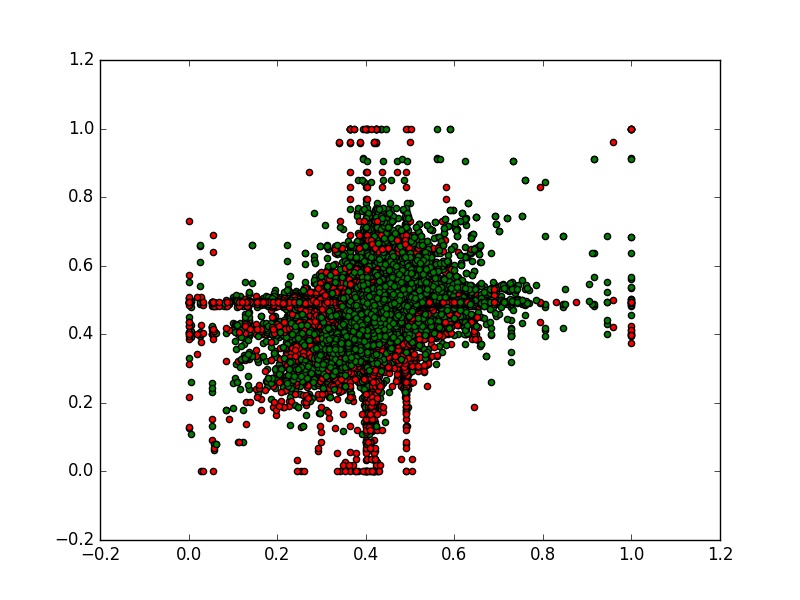
\includegraphics[width=1\columnwidth]{best_2features.jpg}
	\caption{Visualization with 2 Best Features}
	\label{2plot}
\end{figure}
\begin{figure}[H]
	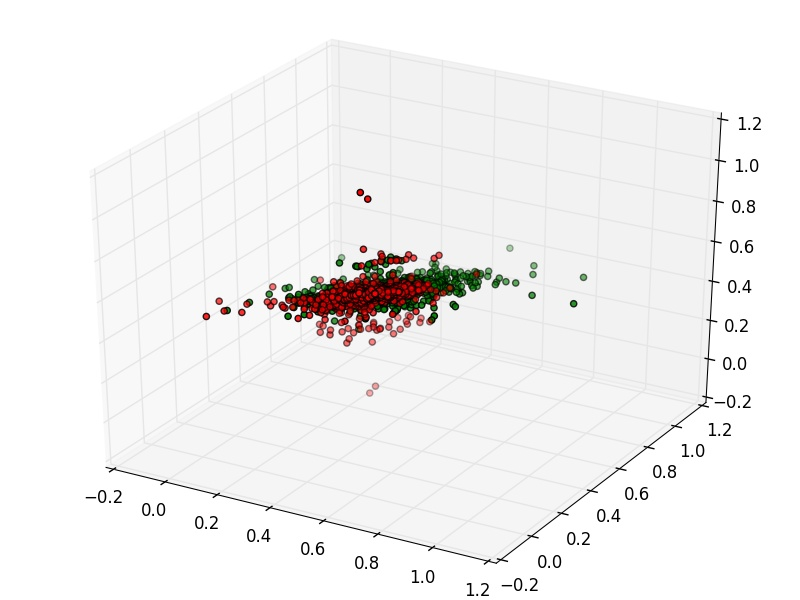
\includegraphics[width=1\columnwidth]{3_6_8viz.jpg}
	\caption{Visualization with 3 Best Features}
	\label{3plot}
\end{figure}	
In order to automate the process, we implemented visualizer functions that consume all possibilities both in 2 and 3 dimensions. Through these methods, data can be visualized with any combination of attributes. In both Figure \ref{2plot} and \ref{3plot}, data is roughly separated with horizontal and vertical planes respectively.\\

Lastly, the training data is composed of 1729 positive instances (occupied) whereas 6414 ones are negative instances (non-occupied). This is a slightly imbalanced dataset, thus considering accuracy would not be a bad choice. Also as a supporting performance metrics, \textit{F1 score} or \textit{gmeans} will possess a complementary role.\\

We have trained several ANNs, SVMs and Decision Trees with different sets of hyper-parameters to compare the estimation rates.

%%%%%%%%%%%%%%%%%%%%%%%%%%%%%%%%%%%%%%%%%%%%%%%%%%%%%%%%%%%%%%

\subsection{Initial Test With Artificial Neural Network}

Our hypothesis states that it is possible to predict occupancy in a space with only using differences in Light level, CO2 level and Humidity level. In order to test the hypothesis, a simple neural network is planned for evaluation.

The proposed initial architecture is a Fully Connected Artificial Neural Network (ANN) which consist of 3 hidden layers. First two hidden layers have 10 neurons each and the last hidden layer have 8 neurons. There is a drop out layer in between second and third hidden layer to combat over fitting. Figure \ref{fig:ann-struct} is an illustration of this setup. The network uses ReLU as activation function for all neurons except last hidden layer which uses Softmax as activation function. It uses a simple Mean Squared Error (MSE) as Loss Function and also uses Adam optimizer \cite{Adam} with learning rate of $0.01$ to optimize it.

\begin{figure}[H]
	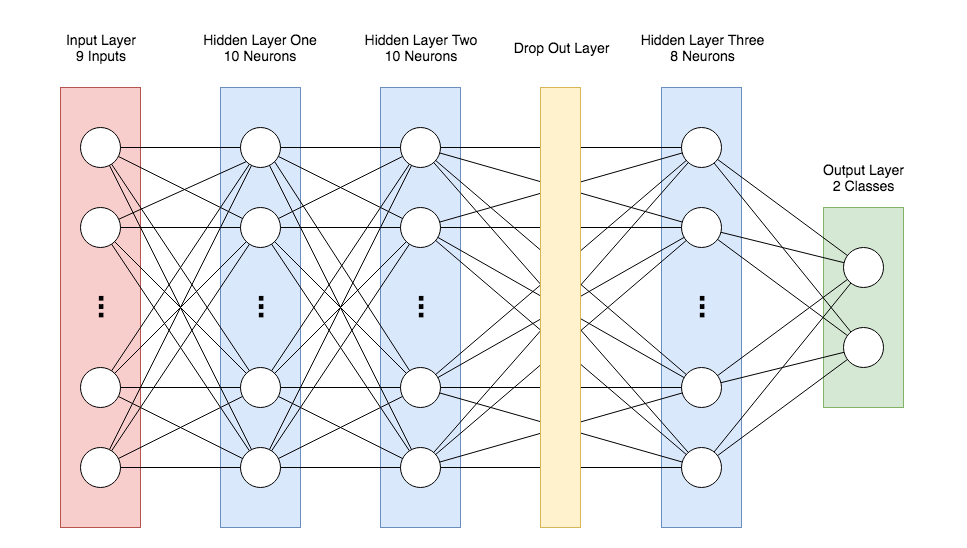
\includegraphics[width=1\columnwidth]{ann-struct.png}
	\caption{Initial structure for the test ANN.}
	\label{fig:ann-struct}
\end{figure}

Tests have been performed on network in different epochs ranging from 500 to 8000. Results of the test are available in Table \ref{tbl-closed-door}. Maximum accuracy is \textbf{0.906} for closed door environment and \textbf{0.81} for open door environment.

\begin{table}[ht]
	\centering
	\caption{Epoch vs. Accuracy of Test Architecture}
	\label{tbl-closed-door}
	\begin{tabular}{|l|l|l|}
		\hline
		\textit{Epochs} & \textit{Accuracy - Closed Door} & \textit{Accuracy - Open Door} \\ \hline
		\textbf{500} & 0.816 & 0.801 \\ \hline
		\textbf{1000} & 0.831 & 0.801 \\ \hline
		\textbf{1500} & 0.888 & \cellcolor{green!25}0.810 \\ \hline
		\textbf{2000} & 0.901 & 0.809 \\ \hline
		\textbf{2500} & 0.899 & 0.807 \\ \hline
		\textbf{3000} & 0.901 & 0.804 \\ \hline
		\textbf{3500} & 0.900 & 0.802 \\ \hline
		\textbf{4000} & 0.904 & 0.805 \\ \hline
		\textbf{4500} & 0.900 & 0.803 \\ \hline
		\textbf{5000} & 0.900 & 0.809 \\ \hline
		\textbf{5500} & 0.897 & 0.805 \\ \hline
		\textbf{6000} & 0.900 & 0.803 \\ \hline 
		\textbf{6500} & \cellcolor{green!25}0.906 & 0.807 \\ \hline
		\textbf{7000} & 0.903 & 0.802 \\ \hline 
		\textbf{7500} & 0.901 & 0.804 \\ \hline
		\textbf{8000} & 0.899 & 0.805 \\ \hline
	\end{tabular}
\end{table}

The high accuracy in this test proves that it is possible to use this augmented data to predict occupancy of an environment. In the next section other methods, architectures and different hyper-parameter optimizations will be attempted.

%%%%%%%%%%%%%%%%%%%%%%%%%%%%%%%%%%%%%%%%%%%%%%%%%%%%%%%%%%%%%%%%

\subsection{Additional Artificial Neural Network Architectures}

In the beginning, a neural network is constructed to initiate experimentation with 2 hidden layers having 10 and 8 hidden units respectively. Input layer contains  9 input units by the number of attributes, whereas output layer contains 2 output units. Learning rate is determined as $\alpha = 0.001$. Loss criterion is \textit{cross entropy} and optimizer function is chosen as \textit{Adam}\footnote{An extension to classical stochastic gradient descent. \href{https://machinelearningmastery.com/adam-optimization-algorithm-for-deep-learning/}{Here} is a nice blog post that explains it in simple terms.} optimizer\cite{Adam}. \textit{Sigmoid} function is the activation function in all layers except the output layer. Output layer employs \textit{softmax} activation function. Loss history is plotted below so as to determine the optimum number of epochs for this particular architecture.\\

\begin{figure}[H]
	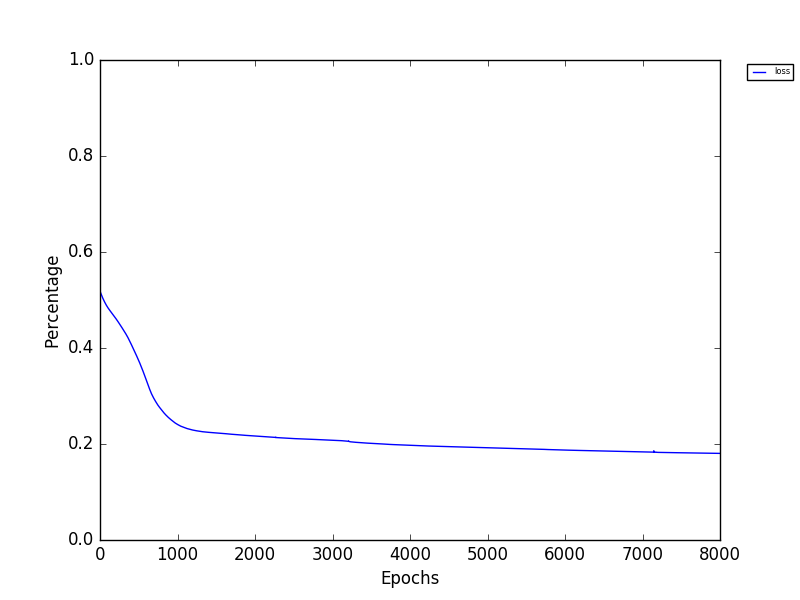
\includegraphics[width=1\columnwidth]{loss_plot.png}
	\caption{Loss History}
	\label{losses}
\end{figure}

As it is seen in the figure \ref{losses} loss number reaches a local minima at roughly 1500 epoches. Since Adam is a variation of Stochastic Gradient Descent, loss does not stabilize and starts producing tiny fluctuations. Stochastic Gradient Descent methods have the ability to recover from local minimum and that is the underlying reason for this phenomenon. Its rate is determined by the nearly extinguished gradients. Therefore, learning process is in proximity of an equilibrium state. Continuing loss reduction only contributes to over-fitting, so learning with high number of epochs will not pay off. Below figure better illustrates the relationship between loss and accuracy/F1 score performance metrics.\\

\begin{figure}[H]
	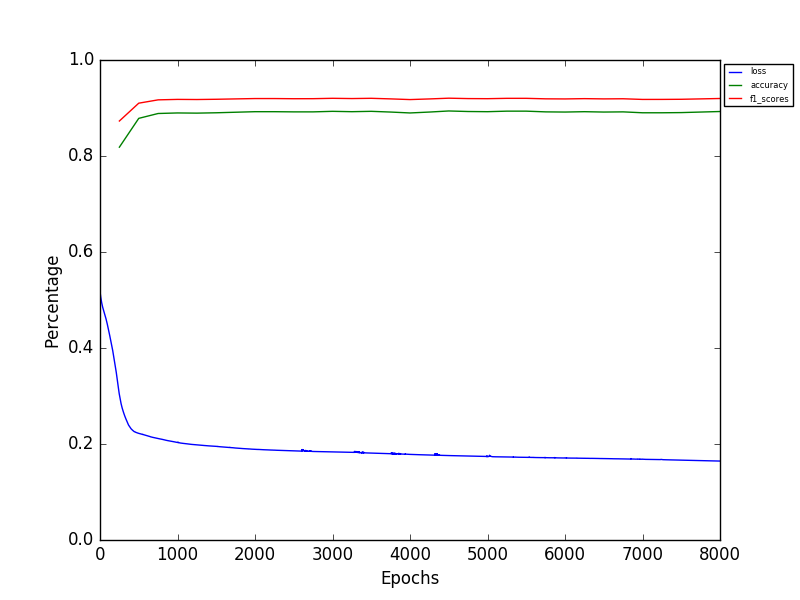
\includegraphics[width=1\columnwidth]{mix_plot.png}
	\caption{Loss, Accuracy, F1 Score of $\alpha = 0.001$}
	\label{mix}
\end{figure}

Maximum accuracy is \textbf{0.8896}, F1 score is \textbf{0.9179} with 3000 epochs. Next experiments are done with the aim of increasing these rates above 90\% instead of just trying all the hyper-parameters na\"ively. In order to determine whether there exists a better minima in the loss function; learning rate should be configured.\\

\begin{figure}[H]
	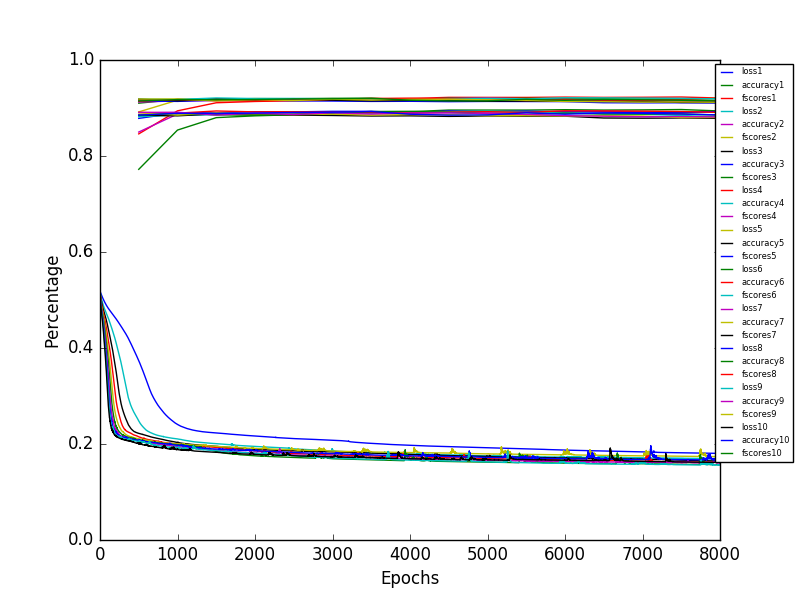
\includegraphics[width=1\columnwidth]{mix_plot_lr.png}
	\caption{Loss, Accuracy, F1 Score of $\alpha \in [0.001 - 0.01]$ with step 0.001} 
	\label{mix_lr}
\end{figure}
Figure \ref{mix_lr} represents loss,  accuracy, F1 score values with respect to learning rates and epochs. \textit{loss1} denotes the loss curve with learning rate 0.001. All subsequent curves are plotted in this manner, i.e. index on right-hand side is multiplied by a factor of 0.001. This set of experiments output \textit{accuracy} and \textit{F1 score} with learning rate $\alpha=0.009$ at epoch 2500 as at most \textbf{0.8961} and \textbf{0.9221} respectively. A very brief and concise comment can be brought about the figure above; that is, as learning rate increases the speed of loss convergence and fluctuations increase, which makes them \textit{relatively bad} models especially with higher number of epochs.\\

Experiments thus far have been done with a simple model. Architecture adjustment is normally required when there are over-fitting or under-fitting issues in the learning process. Nonetheless, this model does not suffer from those two; thus, adjusting the number of layers and their sizes would not make any significant improvements on the estimations. In any case, this assumption should be tested via experimentation on these particular hyper-parameters. Note that learning rate is fixed to 0.009.\\

\begin{table}[H]
	\centering
	\caption{Epoch vs. Accuracy of Several Architectures - Closed Door}
	\label{AllArches}
	\begin{tabular}{|l|l|l|l|l|l|}
		\hline
		& \textit{9x10x10x8x4} 
		& \textit{9x16x8x8x4}
		& \textit{9x10x8x12x4 \textbf{*}}
		& \textit{9}
		& \textit{9x8}\\ \hline
		\textbf{500} & 0.893 & 0.890 & 0.884 & 0.820 & 0.879\\ \hline
		\textbf{1000} & \cellcolor{green!25}0.898 & 0.890 & 0.893 & 0.820 & 0.891\\
		\hline
		\textbf{1500} & 0.894 & 0.886 & 0.896 & 0.820 & 0.892\\ \hline
		\textbf{2000} & 0.892& 0.883 & 0.894 & 0.820 & 0.889\\ \hline
		\textbf{2500} & 0.892 & 0.878 & 0.890 &  0.821 & 0.601\\
		\hline
		\textbf{3000} & 0.894 & 0.879 & 0.887 & 0.821 & 0.878\\ \hline
		\textbf{3500} & 0.894 & 0.878 & 0.888 & 0.821 & 0.885\\ \hline
		\textbf{4000} & 0.890 & 0.875 & 0.885 & 0.821 & 0.880\\ \hline
		\textbf{4500} & 0.893 & 0.874 & 0.886 & 0.821 & 0.880\\ \hline
		\textbf{5000} & 0.893 &  0.872 & 0.885 & 0.821 & 0.883\\ \hline
		\textbf{5500} & 0.892 & 0.874 & 0.884 & 0.821 & 0.879\\ \hline
		\textbf{6000} & 0.890 & 0.875 & 0.884 & 0.821 & 0.882\\ \hline 
		\textbf{6500} & 0.889 & 0.877 & 0.886 & 0.821 & 0.878\\ \hline
		\textbf{7000} & 0.891 & 0.875 & 0.886 & 0.821 & 0.883\\ \hline 
		\textbf{7500} & 0.889 & 0.873 & 0.884 & 0.821 & 0.883\\ \hline
		\textbf{8000} & 0.890 & 0.873 & 0.882 & 0.821 & 0.880\\ \hline
	\end{tabular}
\end{table}
\indent\textbf{*} Hidden layer before the output layer utilizes \textit{ReLU} activation function instead of sigmoid.\\

Except the linear model, all models roughly perform the same as can be seen in the figure. After several experiments, first architecture with 4 hidden layers with respectively 10, 10, 8 and 4 hidden units outputs the best accuracy of \textbf{0.898} at 1000 epochs among other configurations. Reaching such an accuracy rate in shorter training durations is also another advantage.\\

Above experiments serve the base for fine-tuning for overall model to improve and thus only consider first test set which is gathered when the door is closed. A similar table to Table \ref{AllArches} is sketched below for open door test set.\\

Note that, initial architecture which employs different loss criteria and an additional dropout computed  substantially less accuracy rates for open door dataset. This is simply because of the increasing noise in the sensor data when the door is opened.

\vfill
\begin{table}[H]
	\centering
	\caption{Epoch vs. Accuracy of Several Architectures - Opened Door}
	\label{AllArches2}
	\begin{tabular}{|l|l|l|l|l|l|}
		\hline
		& \textit{9x10x10x8x4} 
		& \textit{9x16x8x8x4}
		& \textit{9x10x8x12x4 \textbf{*}}
		& \textit{9}
		& \textit{9x8}\\ \hline
		\textbf{500} & 0.778 & 0.795 & 0.789 & 0.789 & 0.790\\ \hline
		\textbf{1000} & 0.804 & 0.805 & 0.799 & 0.789 & 0.797\\
		\hline
		\textbf{1500} & 0.808 & 0.812 & 0.790 & 0.789 & 0.810\\ \hline
		\textbf{2000} & 0.807& 0.810 & 0.794 & 0.789 & \cellcolor{green!25}0.815\\ \hline
		\textbf{2500} & 0.807 & 0.812 & 0.803 &  0.786 & 0.814\\
		\hline
		\textbf{3000} & 0.804 & 0.810 & 0.801 & 0.789 & 0.814\\ \hline
		\textbf{3500} & 0.802 & 0.807 & 0.799 & 0.787 & 0.808\\ \hline
		\textbf{4000} & 0.801 & 0.804 & 0.798 & 0.786 & 0.803\\ \hline
		\textbf{4500} & 0.798 & 0.801 & 0.798 & 0.785 & 0.803\\ \hline
		\textbf{5000} & 0.793 &  0.798 & 0.797 & 0.785 & 0.800\\ \hline
		\textbf{5500} & 0.792 & 0.799 & 0.793 & 0.784 & 0.795\\ \hline
		\textbf{6000} & 0.790 & 0.801 & 0.792 & 0.783 &  0.794\\ \hline 
		\textbf{6500} & 0.788 & 0.803 & 0.791 & 0.782 & 0.793\\ \hline
		\textbf{7000} & 0.787 & 0.804 & 0.786 & 0.782 & 0.792\\ \hline 
		\textbf{7500} & 0.784 & 0.801 & 0.784 & 0.782 & 0.790\\ \hline
		\textbf{8000} & 0.784 & 0.799 & 0.784 & 0.781 & 0.787\\ \hline
	\end{tabular}
\end{table}

In this set of experiments, last architecture reaches to the best accuracy of \textbf{0.815 }rate among others as can be seen in Table \ref{AllArches2}. Learning rate $\alpha$ is fixed to 0.009 as in the first set of experiments.\\
 
Consequently, initial architecture with MSE loss performs slightly better than the current set of architectures which utilizes cross entropy loss, regarding to the closed door test set. Contrarily, latter performs slightly better than the initial architecture in terms of open door test set. 
\subsection{Suport Vector Machines}
For Support Vector Machine method, we configure the SVM parameters and report their results. We record the results for two performance metrics: accuracy and f-score. F-score is also important for us, because our data set is slightly imbalanced. F-score is a kind of weighted average of precision and recall.

We tried every configuration for hyperparameters like penalty parameter(C), tolerance for stopping criterion, kernel function and gamma(kernel coefficient for kernel functions) while creating Support Vector Machine model. In order to do that we trained a model for each configuration separately and measured accuracy and f-score for it. Our best accuracy results are \%86.4520 for the first test dataset and \%79.8351 for the second test dataset. Our best f-score is same for the best configuration for accuracy in first dataset. However, it is different in second dataset. The best f-score result is \%83.5019 for the first dataset and \%67.3889 for the second dataset.

\begin{table}[H]
	\centering
	\caption{SVM Configurations and Accuracy and F-score Results for the First Test Data}
	\label{AllArches}
	\begin{tabular}{|l|l|l|l|l|l|}
		\hline
		C
		& tol
		& gamma
		& kernel
		& accuracy
		& f-score\\ \hline
		0.320 & 0.013 & 0.108 & rbf & 0.833395 & 0.819084\\ \hline
		0.321 & 0.013 & 0.108 & rbf & 0.833395 & 0.819084\\ \hline
		0.322 & 0.013 & 0.108 & rbf & 0.843771 & 0.819573\\ \hline
		0.323 & 0.013 & 0.108 & rbf & 0.843399 & 0.819084\\ \hline
		0.324 & 0.013 & 0.108 & rbf & 0.843771 & 0.819084\\ \hline
		0.325 & 0.013 & 0.108 & rbf & 0.843771 & 0.819084\\ \hline
		0.326 & 0.013 & 0.108 & rbf & 0.843771 & 0.819689\\ \hline
		0.327 & 0.013 & 0.108 & rbf & 0.864146 & 0.820177\\ \hline
		0.328 & 0.013 & 0.108 & rbf & 0.833771 & 0.819805\\ \hline
		0.329 & 0.013 & 0.108 & rbf & 0.864146 & 0.820177\\ \hline
		0.330 & 0.013 & 0.108 & rbf & 0.843771 & 0.819805\\ \hline
		0.327 & 0.0133 & 0.108 & rbf & 0.864146 & 0.820177\\ \hline
		0.327 & 0.0134 & 0.108 & rbf & 0.864146 & 0.820177\\ \hline
		0.327 & 0.0135 & 0.108 & rbf & 0.864146 & 0.820177\\ \hline
		0.327 & 0.0136 & 0.108 & rbf & 0.864146 & 0.820177\\ \hline
		0.327 & 0.0137 & 0.108 & rbf & 0.864146 & 0.820177\\ \hline 
		0.327 & 0.0138 & 0.108 & rbf & 0.864146 & 0.820177\\ \hline
		0.327 & 0.0139 & 0.108 & rbf & 0.864146 & 0.820177\\ \hline 
		0.327 & 0.0136 & 0.109 & rbf & 0.862273 & 0.818205\\ \hline
		0.327 & 0.0136 & 0.110 & rbf & 0.861896 & 0.817717\\ \hline
		0.327 & 0.0136 & 0.111 & rbf & 0.861896 & 0.817717\\ \hline
		0.327 & 0.0136 & 0.112 & rbf & 0.863020 & 0.819063\\ \hline
		0.327 & 0.0136 & 'auto' & rbf & \cellcolor{green!25}0.864520 & \cellcolor{green!25}0.835019\\ \hline
		0.327 & 0.0136 & 'auto' & linear & 0.740938 & 0.583340\\ \hline
		0.327 & 0.0136 & 'auto' & sigmoid & 0.562589 & 0.435214\\ \hline
	\end{tabular}
\end{table}


\begin{table}[H]
	\centering
	\caption{SVM Configurations and Accuracy and F-score Results for the Second Test Data}
	\label{AllArches}
	\begin{tabular}{|l|l|l|l|l|l|}
		\hline
		C
		& tol
		& gamma
		& kernel
		& accuracy
		& f-score\\ \hline
		0.315 & 0.013 & 0.108 & rbf & 0.777945 & 0.673503\\ \hline
		0.316 & 0.013 & 0.108 & rbf & 0.777945 & 0.673503\\ \hline
		0.317 & 0.013 & 0.108 & rbf & 0.778047 & 0.673708\\ \hline
		0.318 & 0.013 & 0.108 & rbf & 0.777842 & 0.673410\\ \hline
		0.319 & 0.013 & 0.108 & rbf & 0.777739 & 0.673317\\ \hline
		0.320 & 0.013 & 0.108 & rbf & 0.777739 & 0.673429\\ \hline
		0.321 & 0.013 & 0.108 & rbf & 0.777739 & 0.673429\\ \hline
		0.322 & 0.013 & 0.108 & rbf & 0.777842 & 0.673522\\ \hline
		0.323 & 0.013 & 0.108 & rbf & 0.777842 & 0.673522\\ \hline
		0.324 & 0.013 & 0.108 & rbf & 0.777739 & 0.673429\\ \hline
		0.325 & 0.013 & 0.108 & rbf & 0.777739 & 0.673429\\ \hline
		0.317 & 0.0133 & 0.108 & rbf & 0.778047 & 0.673708\\ \hline
		0.317 & 0.0134 & 0.108 & rbf & 0.778047 & 0.673708\\ \hline
		0.317 & 0.0135 & 0.108 & rbf & 0.778047 & 0.673708\\ \hline
		0.317 & 0.0136 & 0.108 & rbf & 0.778047 & 0.673708\\ \hline
		0.317 & 0.0137 & 0.108 & rbf & 0.778047 & 0.673708\\ \hline 
		0.317 & 0.0138 & 0.108 & rbf & 0.778047 & 0.673708\\ \hline
		0.317 & 0.0139 & 0.108 & rbf & 0.778047 & 0.673708\\ \hline 
		0.317 & 0.0136 & 0.109 & rbf & 0.777947 & 0.673503\\ \hline
		0.317 & 0.0136 & 0.110 & rbf & 0.777945 & 0.673503\\ \hline
		0.317 & 0.0136 & 0.111 & rbf & 0.777945 & 0.673503\\ \hline
		0.317 & 0.0136 & 'auto' & rbf & 0.778150 & \cellcolor{green!25}0.673889\\ \hline
		0.317 & 0.0136 & 'auto' & linear & \cellcolor{green!25}0.798351 & 0.546185\\ \hline
		0.317 & 0.0136 & 'auto' & sigmoid & 0.674889 & 0.514299\\ \hline
	\end{tabular}
\end{table}

\subsection{Decision Trees}

The main idea behind the decision tree algorithm is to build a tree-like model from root to leaf nodes. All nodes receive a list of inputs and the root node receives all the examples in the training set. Each node asks a true or false question for a feature and responses by partitioning into two subsets. The subsets then become the input the child nodes where the child node asks another question for one of the other features.\\

The challenge to building such a tree is which question to ask at a node and when. To do this, some experiments were done by tuning some parameter values, such as "Criterion" to measure the quality of a split which can be "gini" for the Gini impurity as a criterion to minimize the probability of misclassification or "entropy" for the information gain i.e. the amount of information that's gained by knowing the value of the entropy of the distribution before subtracted by the entropy of the distribution after the split, "Max Depth" for maximum depth of the tree, "Min Weight" to set the minimum weighted fraction of the sum total of weights required to be at a leaf node, "Max Features" to set the number of features to consider when looking for the best split, and "Random State" for the randomness of the state.   

Below are the tables consists of some experimental data in two cases, closed and open door.

\begin{table}[H]
	\centering
	\caption{Accuracy and F1-Score of Closed Door Case}
	\label{AllArches}
	\begin{tabular}{|p{1cm}|p{0.7cm}|p{0.7cm}|p{0.7cm}|p{1cm}|p{1cm}|p{1cm}|p{1cm}|}
	    \hline
		\textit{Criterion} 
		& \textit{Max Depth}
		& \textit{Min Weight}
		& \textit{Max Features}
		& \textit{Random State}
		& \textit{Accuracy}
		& \textit{F1 Score}\\ \hline
		entropy & None & 0 & auto & 0 & 0.789 & 0.763\\ \hline
		gini & None & 0 & None & None & 0.783 & 0.763\\ \hline
		gini & 4 & 0 & None & None & 0.826 & 0.797\\ \hline
		gini & 6 & 0 & None & None & 0.834 & 0.80\\ \hline
		gini & 7 & 0 & None & None & 0.832 & 0.805\\ \hline
		entropy & 6 & 0 & auto & 0 & 0.822 & 0.790\\ \hline
        entropy & 6 & 0 & sqrt & None & 0.822 & 0.790\\ \hline
        entropy & 6 & 0.01 & log2 & 0 & 0.822 & 0.785\\ \hline
		gini & 6 & 0.5 & None & None & 0.635 & 0.388\\ \hline
        gini & 6 & 0.1 & None & None & 0.809 & 0.763\\ \hline
        gini & 6 & 0.01 & None & None & 0.818 & 0.788\\ \hline
        gini & 6 & 0.01 & auto & None & 0.827 & 0.793\\ \hline
        gini & 6 & 0.01 & sqrt & None & 0.817 & 0.785\\ \hline
        gini & 6 & 0.01 & log2 & None & 0.829 & 0.804\\ \hline
        gini & 6 & 0.01 & 2 & None & 0.823 & 0.792\\ \hline
        gini & 6 & 0 & auto & None & 0.828 & 0.800\\ \hline
        gini & 6 & 0 & sqrt & None & 0.818 & 0.787\\ \hline
        gini & 6 & 0 & log2 & None & 0.826 & 0.790\\ \hline
        gini & 6 & 0 & 2 & None & 0.815 & 0.778\\ \hline
        gini & 6 & 0 & auto & 0 & 0.830 & 0.797\\ \hline
        gini & 6 & 0 & sqrt & 0 & 0.830 & 0.797\\ \hline
        gini & 6 & 0 & log2 & 0 & 0.830 & 0.797\\ \hline
        gini & 6 & 0 & 2 & 0 & \cellcolor{green!25}0.834 & 0.803\\ \hline
	\end{tabular}
\end{table}

As we can see from the table above, we started the experiment by comparing the Criterion function. We got the accuracy better when we use gini function instead of entropy. Focusing on gini function, we iterate to find the best number of the maximum depth of the tree, and find 6 is the best on this case. Then we tune the Min Weight value, and pick 0.0 and 0.1 to be taken for comparison in the continuing experiment. We then try some possible values for Max Features and Random State. As the result, the maximum \textit{accuracy} after training for the case of closed door is \textbf{0.834} with \textit{F1 score} is \textbf{0.803}, when gini criteria was used for the Gini impurity and the maximum depth of the decision tree is 6. \\

For further result to see the tree produced on best accuracy of closed door case, go to this url: \url{https://www.dropbox.com/s/uzmkfe0ugdlzr67/decision_tree_closed_door.png?dl=0}


\begin{table}[H]
	\centering
	\caption{Accuracy and F1-Score of Open Door Case}
	\label{AllArches}
	\begin{tabular}{|p{1cm}|p{0.7cm}|p{0.7cm}|p{0.7cm}|p{1cm}|p{1cm}|p{1cm}|p{1cm}|}
	    \hline
		\textit{Criterion} 
		& \textit{Max Depth}
		& \textit{Min Weight}
		& \textit{Max Features}
		& \textit{Random State}
		& \textit{Accuracy}
		& \textit{F1 Score}\\ \hline
		entropy & None & 0 & auto & 0 & 0.730 & 0.639\\ \hline
        gini & None & 0 & None & None & 0.715 & 0.624\\ \hline
        gini & 4 & 0 & None & None & 0.796 & 0.667\\ \hline
        gini & 6 & 0 & None & None & 0.797 & 0.680\\ \hline
        gini & 7 & 0 & None & None & 0.801 & 0.684\\ \hline
        gini & 7 & 0 & auto & None & 0.795 & 0.672\\ \hline
        gini & 7 & 0 & sqrt & None & 0.791 & 0.665\\ \hline
        gini & 7 & 0 & log2 & None & 0.795 & 0.676\\ \hline
        gini & 7 & 0 & 2 & None & 0.760 & 0.629\\ \hline
        gini & 7 & 0.5 & None & None & 0.798 & 0.673\\ \hline
        gini & 7 & 0.1 & None & None & 0.801 & 0.674\\ \hline
        gini & 7 & 0.01 & None & None & 0.796 & 0.667\\ \hline
        gini & 7 & 0.01 & auto & None & 0.781 & 0.659\\ \hline
        gini & 7 & 0.01 & sqrt & None & 0.784 & 0.660\\ \hline
        gini & 7 & 0.01 & log2 & None & \cellcolor{green!25}0.802 & 0.660\\ \hline
        gini & 7 & 0.01 & 2 & None & 0.775 & 0.661\\ \hline
        gini & 7 & 0.01 & auto & 0 & 0.792 & 0.680\\ \hline
        gini & 7 & 0.01 & sqrt & 0 & 0.792 & 0.680\\ \hline
        gini & 7 & 0.01 & log2 & 0 & 0.792 & 0.680\\ \hline
        gini & 7 & 0.01 & 2 & 0 & 0.784 & 0.646\\ \hline
        entropy & 7 & 0 & auto & 0 & 0.792 & 0.670\\ \hline
        entropy & 7 & 0 & sqrt & None & 0.797 & 0.670\\ \hline
        entropy & 7 & 0.01 & log2 & None & 0.782 & 0.656\\ \hline
	\end{tabular}
\end{table}

While in experiment of the open door case as shown in table above, by doing similar approach as done in previous case, the best \textit{accuracy} obtained is \textbf{0.801} with \textit{F1 score} is \textbf{0.660} when we use gini criterion with maximum depth is 7 and the number of maximum features is the log2 of the number of the features.\\

More, by comparing the "Max Feature" values, we also see that the best accuracy is always obtained when the number of maximum features to consider when looking for the best split is set to be log2 for this dataset. \\

For further result to see the tree produced on best accuracy of open door case, go to this url: \url{https://www.dropbox.com/s/42ncyrdaorvfsuf/decision_tree_opened_door.png?dl=0}

\vspace{2cm}
\section{Conclusion}
The conclusion goes here.




% conference papers do not normally have an appendix


% use section* for acknowledgment
\section*{Acknowledgment}


The authors would like to thank...



\begin{thebibliography}{1}
\bibitem{OccMeasure}
T. Labeodan, W. Zeiler, G. Boxem, Y. Zhao, \emph{\textbf{Occupancy   measurement   in   commercial   office  
buildings   for   demand-driven   control   applications   -   A   survey   and   detection   system   evaluation.}}\\  
Energy and Buildings. 93(2015), pp. 303-314.
\bibitem{ReductoHVAC}
V.   L.   Erickson,   M.   a.   Carreira-Perpinan,   A.   E.   Cerpa,    \emph{\textbf{OBSERVE: Occupancy-based system for efficient reduction of HVAC energy.}}\\Proceedings   of   the   10th   ACM/IEEE   International   Conference  
on Information Processing in Sensor Networks, 258-269 (2011).
\bibitem{SensorOcc}
B.   Dong,   B.   Andrews, \emph{\textbf{Sensor-based   Occupancy   Behavioral   Pattern   Recognition   For   Energy  
And   Comfort   Management   In   Intelligent   Buildings}}\\Eleventh   International   IBPSA   Conference,  
1444-1451 (2009).
\bibitem{TargetCons}
E.U., \emph{\textbf{Directive 2010/31/EU of the European Parliament and of the Council of 19
May 2010 on the Energy Performance of Buildings (Recast)}}, Off. J. Eur. Union
53 (2010) 13-33.
\bibitem{Candanedo}
L. M. Candanedo, V. Feldheim, \emph{\textbf{Accurate occupancy detection of an office room from light, temperature, humidity and CO2 measurements using statistical learning models}}, Energy and Buildings. 112, (2016) 28-39.
\bibitem{Erickson}
V. L. Erickson, M. Á. Carreira-Perpiñán, A. E. Cerpa, \emph{\textbf{Occupancy Modeling and Prediction for Building Energy Management.}} ACM Transactions on Sensor Networks. 10, 1-28 (2014).
\bibitem{Ryu}
S. H. Ryu, H. J. Moon, \emph{\textbf{Development of an occupancy prediction model using indoor environmental data based on machine learning techniques.}} Building and Environment. 107, 1-9 (2016).
\bibitem{Pedersen}
T. H. Pedersen, K. U. Nielsen, S. Petersen, \emph{\textbf{Method for room occupancy detection based on trajectory of indoor climate sensor data.}} Building and Environment. 115, 147-156 (2017).
\bibitem{Guyon}
I. Guyon, A. Elisseeff  \emph{\textbf{An Introduction to Variable and Feature Selection}}
Journal of Machine Learning Research 3  1157-1182 (2003).
\bibitem{Fahim}
M. F. Zibran
\emph{\textbf{CHI-Squared Test of Independence}}
\bibitem{Adam}
D. P. Kingma, J. L. Ba
\emph{\textbf{Adam: A Method for Stochastic Optimization }}
International Conference on Learning Representations (2015).
\end{thebibliography}




% that's all folks
\end{document}


